%======================================================================
\chapter{Conclusion and Future Work}
\label{ch: Chapter6}
%======================================================================
In this work, we presented a project that sucessfully utilized, control theory, embedded development, and mechatronics.  The following sections will overview the accomplishments and provide suggestions for future work.

%----------------------------------------------------------------------
\section{Conclusion}
%----------------------------------------------------------------------
Before we started this project, we did research on different kinds of control algorithms done in previous works and addressed by literature.  We chose to study and implement LQR, LQR, and ADP on the Quanser Aero because we believed that would be the best for an embedded device.\\
Simulations were conducted for two of the three different control algorithms explain in this work: LQR and LQG.  This was done using Simulink and creating a model for our plant.  ADP was already extensively simulated and modeled in last years work.\\
After we were confident our controller was stable and had met our expectations, we used a labortory computer to implement our design.  This utilized a USB connection to send voltage commands to the helicopter and recieve position data.  The results were similar to our simulations, but some changes were needed to be made in order to error. \\
We then began to make adjustments to our design so that it could be implemented on a single board computer.  This required us to change the interface for the helicopter to the Q-flex2 panel.  This method uses SPI communication and is slower than USB.  As a result the preformance slightly dropped.  We were also unable to implement LQG and the PI version of LQR.\\
Once we were ready to move to the mobile device, we had to create a new model to be implemented on the mobile device.  Also, all models now had to recive UDP send packets containg configuration data. 

%%----------------------------------------------------------------------
%\section{Algorithm Comparison}
%%----------------------------------------------------------------------
%The PI type controller greatly reduces steady state error in the experimental results.  ADP works best when the system parameters are unknown or time-variant.  See Chapter~\ref{ch: Chapter5} for an indepth analysis for each individual control algorithm

%----------------------------------------------------------------------
\section{Future Work}
%----------------------------------------------------------------------
This projects has great potential as a learning tool for future students.  This section has prepared a list of improvements that could be encoperated in future work.

\subsection{Enhanced Smart Framework}
For a device to be considered Smart device, it must meet a certian set of criteria.  It must have the ability to interact remotely over a network, respond to user input, and have some degree of autonomy.  Although our framework exhibits these characteristics, there is room to expand upon network connectivity.  Currently, IP address must be manually set before you programs are built and complied.  As more helicopters and controllers are added to the network, the complexity of the mobile device's program will increase.  If too many devices are communicating with the mobile device, it could overload the devices network ability causing effects similar to a denial of service (DoS) attack.\\
To address this issue, future work could be implemented to create a server which would handle the flow of information from the mobile device to the controllers and vice versa as shown in Figure~\ref{fig:Smart_Alg}.  In this case, the mobile device sould send a configuration signal to the server and specify which helicopters or group of helicopters the configuration should be applied to.  This would allow the server to more effeciently manage packets sent and recieved between devices.\\
\begin{figure}[!htbp]
    \centering
    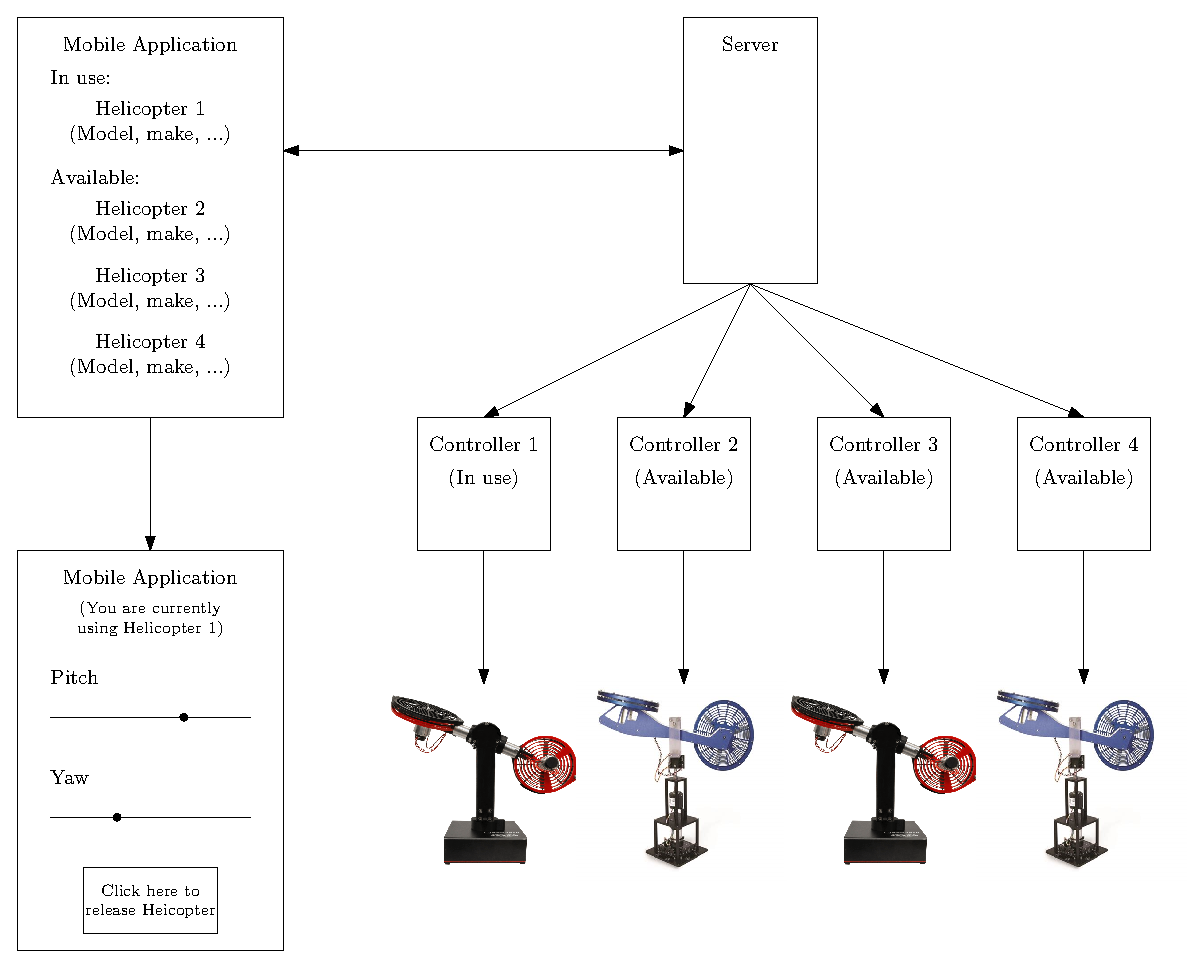
\includegraphics[width=.46\textwidth,keepaspectratio=true]{figs/ipe/smartAlg.eps}
    \label{fig:Smart_Alg}
    \caption{Smart Algorithm Server Connectivity}
\end{figure}
In order to encoperate this kind of connectivity into this framework, it may be necessary to consider a convergence project between electrical engineer and computer science or management information system students.

\subsection{Digital Compass}
When the helicopter is initial turned on, the current configuration is assumed to be the point of origin.  This is because there is not infracture for the helicopter to determine an equilibrium point.  This can cause problems if the user is in a remote location and can not visually confirm the helicopter's heading.  We propose that a digital compass be incorperated into the design of the controller both to assist in determining initial orientation, but also to account for encoder error.  Encoders commonly report error when left running for long periods of time.

\subsection{Expanded PI Control}
This project encountered trouble implementing the PI control architecture as well as LQG on the Raspberry Pi. This may be because the integrator and the kalman filter require a fixed sampling time.  Simulink has the option to use a variable sampling time when set to continuous time.  Since the model is being loaded onto a embedded system which relies upon a fixed sampling time, this may be effecting the values being outputted by these blocks.\\
To correct this issue, we recommend that future work done on this project starts with converting the helicopter model into discrete time.  Consider \ref{eq:discreteA} and \ref{eq:discreteB} to convert the continuous model in \ref{eq:stateModel}:
\begin{equation}
\label{eq:discreteA}
    x(k+1)=\Phi x(k)+\Gamma u(k)+\omega u(k)
\end{equation}
\begin{equation}
\label{eq:discreteB}
    y(k)=Hx(k)+Ju(k)
\end{equation}
where $T$ is the sampling time, $\Phi=e^{AT}$, and $\Gamma=\int_0^T e^{A\eta} d\eta B$.\\
This project also did not create a PI version for ADP.  Future work should also explore this architecture as based on the results discussed in this paper, it is likely that it will prove to be the best control algorithm for this platform.

%----------------------------------------------------------------------



%%% Local Variables:
%%% mode: latex
%%% TeX-master: "../finalReport"
%%% End:
